\documentclass[11pt]{article}
\usepackage[T1]{fontenc}
\usepackage{lmodern}
\usepackage[margin=1in]{geometry}
\usepackage{amsmath,amssymb,amsthm,mathtools}
\usepackage{microtype}
\usepackage{needspace}
\usepackage{enumitem}
\usepackage{booktabs}
\usepackage{xcolor}
\usepackage{xurl}
\usepackage{tikz}
\usetikzlibrary{arrows.meta,positioning,calc,decorations.pathreplacing}
\usepackage{cite}
\usepackage[colorlinks=true,linkcolor=blue!50!black,citecolor=blue!50!black,urlcolor=blue!50!black]{hyperref}
\usepackage{bookmark}
\usepackage[capitalise,noabbrev,nameinlink]{cleveref}
\hypersetup{pdftitle={Diagonal Fourier extension for positively curved surfaces in three dimensions},pdfauthor={OpenAI}}
\newtheorem{theorem}{Theorem}[section]
\newtheorem{proposition}[theorem]{Proposition}
\newtheorem{lemma}[theorem]{Lemma}
\newtheorem{corollary}[theorem]{Corollary}
\theoremstyle{definition}
\newtheorem{definition}[theorem]{Definition}
\newtheorem{remark}[theorem]{Remark}
\numberwithin{equation}{section}
\newcommand{\R}{\mathbb R}
\newcommand{\Z}{\mathbb Z}
\newcommand{\C}{\mathbb C}
\newcommand{\N}{\mathbb N}
\newcommand{\eps}{\varepsilon}
\newcommand{\dd}{\,d}
\DeclareMathOperator{\supp}{supp}
\DeclareMathOperator{\diam}{diam}
\DeclareMathOperator{\dist}{dist}
\setlist[enumerate]{label=\textup{(\roman*)},leftmargin=*}
\setlist[itemize]{leftmargin=*}
\title{Diagonal Fourier extension for positively curved surfaces\\in three dimensions}
\author{OpenAI}
\date{September 24, 2026}
\begin{document}
\maketitle
\begin{abstract}
We prove the diagonal Fourier extension conjecture for compact smooth
positively curved surfaces \(\Sigma\subset\R^3\), including surfaces with
smooth boundary. For every \(3<p<\infty\), the extension operator maps
\(L^p(\Sigma)\) boundedly into \(L^p(\R^3)\).
The compact paraboloid case also yields free Schr\"odinger local smoothing
in two spatial dimensions for every \(3<p<\infty\) and Sobolev order
\(s>2-6/p\).
\end{abstract}
\providecommand{\PacketTheoremNumber}{6.4}
\providecommand{\PacketBoundEquation}{6.8}
\providecommand{\PacketPhaseSection}{6.1}
\providecommand{\PacketFamilyDefinition}{6.3}
\providecommand{\PacketProofSection}{7}

\section{Introduction}\label{sec:introduction}

Let \(\Sigma\subset\R^3\) be a compact smooth surface, with induced
surface measure \(d\sigma\). Its Fourier extension operator is
\[
 E_\Sigma f(x)=\int_\Sigma f(\xi)e^{2\pi i x\cdot\xi}\dd\sigma(\xi).
\]
We allow smooth boundary. Positive curvature means that the second
fundamental form is definite at every point, with the normal chosen
on each chart so that the form is positive definite.

\begin{theorem}\label{thm:main}
Let \(\Sigma\subset\R^3\) be a compact smooth positively curved
surface, possibly with smooth boundary. For every \(3<p<\infty\),
there is a finite constant \(C_{\Sigma,p}\) such that
\begin{equation}\label{eq:main}
 \|E_\Sigma f\|_{L^p(\R^3)}
 \le C_{\Sigma,p}\|f\|_{L^p(\Sigma)}
\end{equation}
for every complex-valued \(f\in L^p(\Sigma)\).
\end{theorem}

The theorem establishes the diagonal extension conjecture in three
dimensions for positively curved surfaces. It includes the sphere,
compact elliptic paraboloid patches, and general smooth elliptic
graphs. The surface and the exponent are fixed throughout each
estimate.

\paragraph{Background.}
The restriction problem originates in Stein's work; the
Tomas--Stein theory gives \(L^2(\Sigma)\to L^4(\R^3)\)
for positively curved surfaces \cite{Tomas1975,Stein1979}.
The bilinear framework of Tao, Vargas, and Vega
\cite{TaoVargasVega1998}, Wolff's cone estimate \cite{Wolff2001},
and Tao's paraboloid estimate \cite{Tao2003} developed the role of
wave packets and transverse interactions. Bennett, Carbery, and Tao's
multilinear estimates \cite{BennettCarberyTao2006} and
Bourgain--Guth's approach \cite{BourgainGuth2011} further connected
these interactions to the linear problem.

Guth's polynomial-partitioning argument
established the bounded-data estimate for \(p>13/4\)
\cite[Theorem~0.1]{Guth2016}. Shayya obtained diagonal estimates in that range
\cite[Corollary~2.1(iii)]{Shayya2017}; see also Kim's treatment
\cite[Theorem~1.2 and the following remark]{Kim2017}. Wang's broom
method further improved bounded-data restriction for the truncated
paraboloid \cite[Theorem~1.4]{Wang2022Brooms}. Wang and Wu proved
the diagonal bound for \(p>22/7\) on compact positively curved
surfaces, including surfaces with boundary, using decoupling and
two-ends Furstenberg inequalities \cite[Theorem~0.2]{WangWu2024}.

For the sphere and quadratic graphs, factorization gives a separate
route from bounded-data estimates to diagonal estimates with an
arbitrarily small increase in the exponent; see
Bourgain \cite{Bourgain1991Besicovitch} and Buschenhenke
\cite[Theorem~1.1 and Remark~1.6]{Buschenhenke2024}. The argument here treats general smooth
elliptic charts through the packet theorem's full array formulation
and the explicit phase continuation. The packet and maximal inputs
play distinct roles: the former controls oscillatory coefficients,
while the latter controls their positive tube density.

The compact paraboloid case also gives a consequence for free
Schr\"odinger evolution. Let \(W^{s,p}(\R^2)\) denote the inhomogeneous
Bessel-potential space with norm
\(\|f\|_{W^{s,p}}=\|(I-\Delta)^{s/2}f\|_{L^p(\R^2)}\).

\begin{corollary}[Free Schr\"odinger local smoothing]\label{cor:schrodinger-smoothing}
For every \(3<p<\infty\) and \(s>2-6/p\), the free Schr\"odinger
propagator, initially defined on Schwartz functions, extends boundedly
from \(W^{s,p}(\R^2)\) to \(L^p(\R^2\times[0,1])\):
\begin{equation}\label{eq:schrodinger-smoothing}
 \|e^{it\Delta}f\|_{L^p(\R^2\times[0,1])}
 \le C_{p,s}\|f\|_{W^{s,p}(\R^2)}.
\end{equation}
\end{corollary}

The spacetime norm is global in space and local in time. Rogers's necessary
condition \cite[Section~2]{Rogers2008} shows that the Sobolev threshold
cannot be lowered. We deduce the corollary from the compact-frequency
transfer of Lee, Rogers, and Seeger \cite[Theorem~1.1]{LeeRogersSeeger2013}
in Section~\ref{sec:surfaces}.

A second consequence concerns local oscillatory integrals with phase
\(N[x\cdot y+\psi(t;y)]\), where \(x,y\in\R^2\), \(t\in\R\),
and the amplitude is smooth and compactly supported. Suppose
\(D_y^2\partial_t\psi\) is definite and its time derivative is a
scalar multiple of itself. A change of output variables then reduces
the phase to a fixed elliptic graph. Corollary~\ref{cor:bourgain-oscillatory}
gives the resulting \(L^p\) estimate with the scaling factor
\(N^{-3/p}\) for every finite \(p>3\). The additional phase condition
is the translation-invariant form of Bourgain's condition; we explain
the straightening directly in Section~\ref{sec:surfaces}, following
the setting of Gao--Liu--Xi \cite{GaoLiuXi2025}.

The proof of Theorem~\ref{thm:main} uses two theorem inputs. The packet
propagation theorem \cite[Theorem~\PacketTheoremNumber]{OpenAIPacket2026}
controls
arbitrary finite complex coefficient arrays through an elliptic
capacity, with coordinate masks permitted. The Kakeya maximal
theorem \cite[Theorem~1.1]{OpenAIKakeya2026} controls nonnegative
weighted tube concentration. We state both inputs in the forms used
here and verify their hypotheses. The remainder of the proof gives
the density conversion, the estimates for rough \(L^3\) graph data,
and the passage to general surfaces.

\paragraph{The argument.}
After fixing a graph chart, an explicit continuation places its
phase in the class allowed by the packet theorem. The construction
matches the quadratic Taylor data in a transition annulus of a
continued spherical patch and preserves uniform ellipticity.
It applies equally to boundary charts, where the graph extends
smoothly and the datum is extended by zero.

The packet theorem gives a cubic sample estimate with a small
spatial power loss and an elliptic-capacity factor. A decomposition
according to the capacity of the remaining coefficients allows this
factor to be summed using the positive weighted tube estimate.
The latter follows from the Kakeya maximal theorem by duality;
its direction and position formulation follows the classical
weighted tube framework of Tao, Vargas, and Vega
\cite[arXiv version~1, Section~3]{TaoVargasVega1998}.

To pass to \(L^3\) data, we prove one joint estimate for a sparse
family of balls. Removing a small union of frequency resonances
makes the corresponding packet analyses almost orthogonal. The
bound is uniform in the ball locations and in arbitrarily large
separations. A covering of each level set then removes the spatial
loss. This follows Tao's sparse-ball strategy for epsilon removal
\cite{Tao1999Epsilon};
see the detailed treatments in Bourgain--Guth's appendix
\cite{BourgainGuth2011} and Kim's appendix \cite{Kim2017}.
We prove the precise covering and summation needed for the present
estimate.

The resulting graph bound has \(L^3\) input and \(L^p\) output
for every \(p>3\). A finite chart decomposition, with the surface
and physical-space Jacobians retained, gives
Equation~\eqref{eq:main} by the finite-measure embedding
\(L^p(\Sigma)\subset L^3(\Sigma)\).

Figure~\ref{fig:argument-map} records the two inputs and the successive
reductions.

\begin{figure}[tbp]
\centering
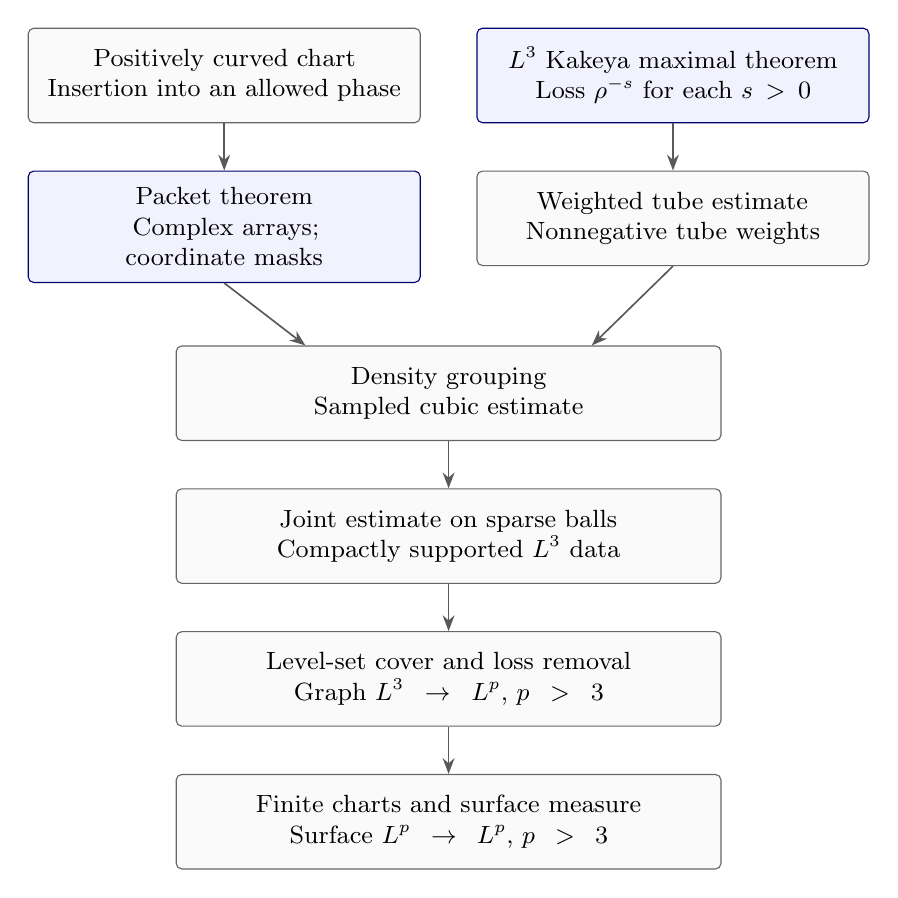
\begin{tikzpicture}[
  font=\small,
  amap box/.style={
    draw=black!60, fill=black!2, rounded corners=2pt,
    align=center, text width=.37\textwidth,
    inner xsep=7pt, inner ysep=6pt, minimum height=12mm
  },
  amap input/.style={amap box, draw=blue!45!black, fill=blue!5},
  amap result/.style={amap box, text width=.53\textwidth},
  amap arrow/.style={-{Stealth[length=2mm]}, draw=black!65, semithick}
]
\node[amap box] (phase) at (-.235\textwidth,0)
  {Positively curved chart\\Insertion into an allowed phase};
\node[amap input] (kakeya) at (.235\textwidth,0)
  {$L^3$ Kakeya maximal theorem\\Loss $\rho^{-s}$ for each $s>0$};

\node[amap input, below=6mm of phase] (packet)
  {Packet theorem\\Complex arrays; coordinate masks};
\node[amap box, below=6mm of kakeya] (tubes)
  {Weighted tube estimate\\Nonnegative tube weights};

\coordinate (join) at ($(packet.south)!.5!(tubes.south)$);
\node[amap result, below=9mm of join] (samples)
  {Density grouping\\Sampled cubic estimate};
\node[amap result, below=6mm of samples] (sparse)
  {Joint estimate on sparse balls\\Compactly supported $L^3$ data};
\node[amap result, below=6mm of sparse] (global)
  {Level-set cover and loss removal\\Graph $L^3\to L^p$, $p>3$};
\node[amap result, below=6mm of global] (surface)
  {Finite charts and surface measure\\Surface $L^p\to L^p$, $p>3$};

\draw[amap arrow] (phase) -- (packet);
\draw[amap arrow] (kakeya) -- (tubes);
\draw[amap arrow] (packet.south) -- ([xshift=-.15\textwidth]samples.north);
\draw[amap arrow] (tubes.south) -- ([xshift=.15\textwidth]samples.north);
\draw[amap arrow] (samples) -- (sparse);
\draw[amap arrow] (sparse) -- (global);
\draw[amap arrow] (global) -- (surface);
\end{tikzpicture}
\caption{The two independent inputs meet in the sampled cubic estimate.
The sparse-ball bound then supplies the common $L^3$ control needed for
globalization and passage to the surface.}
\label{fig:argument-map}
\end{figure}


\paragraph{Dependence on the exponent.}
Let \(C_{\Sigma,p}^{\mathrm{best}}\) denote the operator norm in
Equation~\eqref{eq:main}. Write \(M(s)\ge1\) for the constant in
the Kakeya maximal estimate with loss \(\delta^{-s}\), and let
\(P_\Sigma(\kappa,\eta)\ge1\) be the largest packet constant
among the finitely many fixed chart and window setups used below.
For \(3<p\le4\), put \(\theta=10^{-6}(p-3)^2\). The proof gives
\begin{equation}\label{eq:quantitative-intro}
 C_{\Sigma,p}^{\mathrm{best}}
 \le C(\Sigma)(p-3)^{-7/p}
 P_\Sigma(\theta,\theta)^{1/p}M(\theta)^{3/(2p)},
\end{equation}
where \(C(\Sigma)\) is independent of \(p\in(3,4]\).
The two input theorems supply finite constants at each positive
loss exponent. No rate for their growth is assumed, so
Equation~\eqref{eq:quantitative-intro} records the elementary
losses without asserting a polynomial bound in \((p-3)^{-1}\).
For nonempty \(\Sigma\), a fixed smooth datum also gives
\begin{equation}\label{eq:lower-intro}
 C_{\Sigma,p}^{\mathrm{best}}
 \ge c(\Sigma)(p-3)^{-1/p},\qquad 3<p\le4.
\end{equation}
Proposition~\ref{prop:lower} proves this comparison.

\paragraph{Conventions and organization.}
Write \(e(t)=\exp(2\pi i t)\). All functions and coefficient
arrays may be complex-valued. Constants may depend on the fixed
surface, charts, frequency supports, and windows; dependence on
the small loss exponents is displayed through \(P\) and \(M\).
Section~\ref{sec:setup} fixes the local graph problem. The next
sections give the packet interface, the density conversion, and
the joint sparse-ball estimate. The global argument tracks the
dependence on \(p\), and Section~\ref{sec:surfaces} completes
the transfer to \(\Sigma\) and proves the local-smoothing and
oscillatory-integral consequences.

\section{Local graphs and fixed parameters}\label{sec:setup}

We first explain the class of graph integrals to be estimated.
Near each point of \(\Sigma\), choose tangent coordinates and a
normal in which the surface is a graph with positive definite
Hessian. At a boundary point, a smooth parametrization up to the
boundary extends to an open neighborhood of the parameter
half-disk; this is the usual smooth-boundary convention
\cite[Chapter~1, pp.~27--28]{Lee2013Smooth}. Projection onto the tangent plane has invertible
differential there. The inverse function theorem on the extension
therefore gives a graph on an open planar neighborhood, whose
restriction parametrizes the original surface piece.

After shrinking a chart, Lemma~\ref{lem:continuation} gives a fixed
invertible affine change of ambient frequency coordinates in which
the graph agrees locally with a phase \(\phi\in C^\infty(\R^2)\)
in the precise continuation class of Theorem~\ref{thm:packet}.
In particular, this phase satisfies
\begin{equation}\label{eq:ellipticity}
 cI\le D^2\phi\le CI,\qquad
 \sup_{\R^2}|D^j\phi|<\infty\quad(j\ge2).
\end{equation}
The elementary arguments below use only
Equation~\eqref{eq:ellipticity}; the packet estimate also uses the
continuation form verified in Lemma~\ref{lem:continuation}.

Fix a smooth nonnegative function \(\chi\) supported in a square
centered at zero, such that
\begin{equation}\label{eq:window-partition}
 \sum_{\nu\in a\Z^2}(\chi_a^\nu(\xi))^2=1,\qquad
 \chi_a^\nu(\xi)=\chi((\xi-\nu)/a),\qquad a>0.
\end{equation}
For example, start with a compactly supported bump positive on
\([-1,1]^2\), and divide it by the square root of the sum of the
squares of its integer translates. This denominator is smooth,
positive, and periodic. Let \(D_{\mathrm f}\ge1\) be a fixed side
length for a square containing the support of \(\chi\).

Write
\[
 E_\phi g(y)=\int_{\R^2}g(\xi)
       e\bigl(y'\cdot\xi+y_3\phi(\xi)\bigr)\dd\xi,
 \qquad y=(y',y_3)\in\R^2\times\R.
\]
A partition at scale one reduces each compactly supported graph
integral to finitely many functions of the form
\begin{equation}\label{eq:local-F}
 F(y)=E_\phi(h\chi_1^{\nu_*})(y).
\end{equation}
Here \(\nu_*\in\Z^2\) is fixed and \(h\in L^3(\R^2)\) is supported
in a fixed compact set \(Q_0\). To see the reduction, write graph
data \(g=\sum_{\nu_*}(g\chi_1^{\nu_*})\chi_1^{\nu_*}\), using
Equation~\eqref{eq:window-partition}; only finitely many terms meet
\(\supp g\). The extra copy of the window is included in \(h\).

All constants for a fixed setup may depend on \(\phi,Q_0,\chi\),
\(D_{\mathrm f}\), and \(\nu_*\). These objects, and all label ranges
used later, are chosen before the large scale or the small loss
exponents vary. In particular,
\begin{equation}\label{eq:velocity-monotonicity}
 (\nabla\phi(\xi)-\nabla\phi(\eta))\cdot(\xi-\eta)
 \ge c|\xi-\eta|^2
\end{equation}
on \(\R^2\). Thus the velocity map \(U_\xi=-\nabla\phi(\xi)\) is
bi-Lipschitz on each fixed bounded region and has bounded size there.

The final graph estimate controls Equation~\eqref{eq:local-F} by
\(\|h\|_3\). We record the precise surface Jacobians in
Section~\ref{sec:surfaces}.

\section{The packet estimate and its phase class}\label{sec:packets}

We need a cubic bound for the samples obtained by synthesizing a
finite packet array and analyzing it at a larger scale. The input
array must remain arbitrary, since Section~\ref{sec:density} splits
it into coordinate subarrays. We first verify the precise phase
requirement of the cited packet theorem: uniform convexity alone
is not its stated hypothesis.

\subsection{Continued phases and local changes of coordinates}

The setup of \cite[Section~\PacketPhaseSection]{OpenAIPacket2026} starts with a
small spherical graph and extends its phase smoothly to
$\mathbb R^2$, with uniformly definite bounded Hessian and bounded
derivatives of every order at least two.  Its constants may depend on
this fixed continuation, the fixed bounded frequency region, and the
windows.  The continuation is made by cutting off the difference
from the quadratic Taylor polynomial.  We shall use continuations of
precisely this form: write
\[
 q_s(\xi)=-\sqrt{1-|\xi|^2},\qquad
 Q_s(\xi)=-1+\tfrac12|\xi|^2,
\]
and, for a sufficiently small fixed $\rho>0$, set
\begin{equation}\label{eq:spherical-continuation}
 \phi=Q_s+\zeta(q_s-Q_s),
 \qquad
 0\le\zeta\le1,\quad
 \zeta=1\ \text{on }B(0,\rho),\quad
 \operatorname{supp}\zeta\subset B(0,2\rho).
\end{equation}
Here $\zeta$ is smooth, the product is extended by zero outside
$B(0,2\rho)$, and the resulting phase must satisfy
Equation~\eqref{eq:ellipticity}.  No radiality is required of the cutoff.

\Needspace{5\baselineskip}
\begin{lemma}[Insertion of an elliptic graph]\label{lem:continuation}
Every germ of a smooth graph with positive definite Hessian can be
carried by an invertible affine transformation of $\mathbb R^3$ to a
graph agreeing, on an open neighborhood, with a phase of the form in
Equation~\eqref{eq:spherical-continuation}.  The phase, the neighborhood, and
the affine transformation can all be fixed independently of the
packet scales and of the exponents used below.
\end{lemma}

\begin{proof}
Choose a smooth cutoff $\zeta_0$ equal to one on $B(0,\rho)$,
supported in $B(0,2\rho)$, and identically $1/2$ on a neighborhood
$V$ of a point $\xi_1$ with $\rho<|\xi_1|<2\rho$.
It can be chosen by rescaling a fixed cutoff with an annular plateau.
The phase
\[
 q=Q_s+\zeta_0(q_s-Q_s)
\]
has Hessian $I+O(\rho^2)$: the remainder $q_s-Q_s$ and its
derivatives of orders zero, one, and two are respectively
$O(\rho^4)$, $O(\rho^3)$, and $O(\rho^2)$ on the support of the
cutoff.  Fix $\rho$ small enough that $q''$ is positive definite
everywhere.

After translating the target base point, let its height function be
$h_0$ near zero and put $H=h_0''(0)>0$ and $B=q''(\xi_1)>0$.
Choose an invertible real matrix $A$ with $A^{\mathsf T}HA=B$;
for example, $A=H^{-1/2}B^{1/2}$.  Define, near $\xi_1$,
\begin{align*}
 \psi(\xi)
 &=h_0\bigl(A(\xi-\xi_1)\bigr)+q(\xi_1)-h_0(0)\\
 &\quad+
 \bigl(\nabla q(\xi_1)-A^{\mathsf T}\nabla h_0(0)\bigr)
                \cdot(\xi-\xi_1).
\end{align*}
Thus $\psi$ and $q$ have the same value, gradient, and Hessian at
$\xi_1$.  This change of graph is induced by an invertible affine
map of ambient frequency space: its base part is
$x\mapsto \xi_1+A^{-1}x$, and its height part is addition of an
affine function of the new base coordinates.

Let $\vartheta\in C_c^\infty(B(0,2))$ equal one on $B(0,1)$ and
take $0\le\vartheta\le1$.  For a small fixed $\epsilon>0$ put
\[
 R_\epsilon(\xi)=
 \vartheta\bigl((\xi-\xi_1)/\epsilon\bigr)
                  \bigl(\psi(\xi)-q(\xi)\bigr).
\]
Choose $\epsilon$ so that its support is contained in $V$ and the
target graph is defined there.  Taylor's theorem and the agreement
of the two-jets give
\[
 \|D^jR_\epsilon\|_\infty\le C\epsilon^{3-j},
 \qquad j=0,1,2.
\]
Consequently $\phi=q+R_\epsilon$ remains uniformly convex for
sufficiently small $\epsilon$ and agrees with $\psi$ on
$B(\xi_1,\epsilon)$.  It equals $Q_s$ outside a compact set, so
all of its derivatives of order at least two are bounded.

To verify the required continuation form, observe that
$D=q_s-Q_s$ is strictly positive for $0<|\xi|<1$.
Shrink $V$, if necessary, so that $D\ge d_0>0$ there.  The function
$R_\epsilon/D$, extended by zero outside $V$, is smooth.  Set
\[
 \widetilde\zeta=\zeta_0+R_\epsilon/D.
\]
On the perturbation support, $\zeta_0=1/2$ and
$|R_\epsilon/D|\le C\epsilon^3/d_0$.  Choosing $\epsilon$
smaller makes this last quantity at most $1/4$.  Hence
$0\le\widetilde\zeta\le1$, with the same inner and outer support
properties as $\zeta_0$, and
$\phi=Q_s+\widetilde\zeta(q_s-Q_s)$.
Every choice was made using only the fixed target graph.
\end{proof}

In what follows, the phases to which the cited packet theorem is
applied are chosen as in Lemma~\ref{lem:continuation}.  Although the
inserted graph lies in the transition annulus, the packet theorem
allows arbitrary frequency labels in a fixed bounded region.  In
particular, those labels need not lie in the spherical region
$B(0,\rho)$: \cite[Definition~\PacketFamilyDefinition]{OpenAIPacket2026} imposes
no such restriction, and its single-step maps act on arbitrary
finite input arrays.  All windows meeting the inserted graph, and
the terminal windows used below, can therefore be included in one
fixed bounded frequency region.  The constants may depend on the
chosen phase, including its higher derivative bounds.

\subsection{Frames and the capacity norm}

We use the standard frequency and spatial localization of wave
packets; see Tao \cite[arXiv version~2, Section~4]{Tao2003} and the Fourier-series
construction of Guo, Oh, Wang, Wu, and Zhang
\cite[arXiv version~1, Section~4.1]{GOWWZ2025Packets}. Square windows give the exact
identities below, with the normalization needed for our sample sum.

Fix a dyadic $N\ge2$ and put $\delta=N^{-1}$ and
$U_\nu=-\nabla\phi(\nu)$.  For a dyadic factor $1\le m\le N$ let
\begin{equation}\label{eq:packet-scales}
 \theta=m\delta,\qquad r=m^{-2},\qquad
 w=r\theta=\delta/m.
\end{equation}
Partition $[0,1)$ into intervals $I$ of length $r$, with left
endpoints $t_I$.  At this scale, the indices are
\[
 (\nu,z,I),\qquad
 \nu\in\theta\mathbb Z^2,\qquad
 z\in D_{\mathrm f}^{-1}w\mathbb Z^2.
\]
Using the windows fixed in the local setup, define
\begin{align}
 (\mathsf P_{m,I}f)_{\nu,z}
 &=\int f(\xi)\chi_\theta^\nu(\xi)
              e\bigl(N^2(z\cdot\xi+t_I\phi(\xi))\bigr)\,d\xi,
              \label{eq:packet-analysis}\\
 \mathsf S_{m,I}d(\xi)
 &=(D_{\mathrm f}\theta)^{-2}
   \sum_{\nu,z}d_{\nu,z}\chi_\theta^\nu(\xi)
              e\bigl(-N^2(z\cdot\xi+t_I\phi(\xi))\bigr).
              \label{eq:packet-synthesis-general}
\end{align}
Synthesis is initially defined for finite arrays and then extended
continuously to $\ell^2$.

\begin{lemma}[Exact frame identities]\label{lem:packet-frame}
For every $f\in L^2(\mathbb R^2)$,
\begin{equation}\label{eq:packet-frame}
 \mathsf S_{m,I}\mathsf P_{m,I}f=f,
 \qquad
 \|\mathsf P_{m,I}f\|_{\ell^2}^2
       =(D_{\mathrm f}\theta)^2\|f\|_2^2,
 \qquad
 \|\mathsf S_{m,I}\|_{\ell^2\to L^2}
       =(D_{\mathrm f}\theta)^{-1}.
\end{equation}
\end{lemma}

\begin{proof}
Since $N^2w\theta=1$, the vectors $N^2z$ run through
$(D_{\mathrm f}\theta)^{-1}\mathbb Z^2$.  For each fixed
$\nu$, Equation~\eqref{eq:packet-analysis} is the Fourier
coefficient array of
$f\chi_\theta^\nu e(N^2t_I\phi)$ on a square of side
$D_{\mathrm f}\theta$.  Parseval and Fourier inversion give
\[
 \sum_z|(\mathsf P_{m,I}f)_{\nu,z}|^2
   =(D_{\mathrm f}\theta)^2\|f\chi_\theta^\nu\|_2^2
\]
and, after synthesis, $f(\chi_\theta^\nu)^2$.
Sum over $\nu$ and use $\sum_\nu(\chi_\theta^\nu)^2=1$.
The norm of synthesis follows from
$\mathsf S_{m,I}=(D_{\mathrm f}\theta)^{-2}\mathsf P_{m,I}^*$.
These identities first hold for finite partial Fourier sums in
$L^2$ and then for their limits.
\end{proof}

For $0<\kappa<1/10$, let $E$ be a centered closed ellipse with
ordered semiaxes $L\ge a>0$, of any orientation, and write
$W_\kappa(E)=L^{1+\kappa}a^{1-\kappa}$.
For a finite array $c$ in one bin at the scale
$(\theta,r,w)$ define
\begin{align}
 K_{\theta,r}(c)
 &=\sup_{\substack{E,u,v\\L\ge a\ge\theta}}
   \frac{\theta^2}{W_\kappa(E)}
   \sum_{\substack{U_\nu\in u+E\\z\in v+rE}}|c_{\nu,z}|^2,
                 \label{eq:packet-general-capacity}\\
 G_{\theta,r}(c)^3
 &=\left(w^2\sum_{\nu,z}|c_{\nu,z}|^2\right)
                          K_{\theta,r}(c)^{1/2}.
                 \label{eq:packet-gauge}
\end{align}
The translations $u,v\in\mathbb R^2$ are independent, and there
is no upper restriction on either semiaxis.  On each finite index
set let
\begin{align*}
 A_{\theta,r}(c)&=
 \inf\left\{\sum_{\ell=1}^qG_{\theta,r}(a_\ell):
       |c|\le\sum_{\ell=1}^q|a_\ell|,\ q<\infty\right\},\\
 \mathcal A_m(c)^3&=r\sum_I A_{\theta,r}(c_I)^3.
\end{align*}
The domination in this infimum is coordinatewise.

\Needspace{5\baselineskip}
\begin{lemma}[The atomic norm controls the sample sum]
\label{lem:packet-atomic}
The function $A_{\theta,r}$ is a norm on every finite coordinate
space, is monotone under absolute coordinatewise domination, and
is contracted by coordinate masks.  Moreover,
\begin{equation}\label{eq:packet-atomic-lower}
 rw^2\sum_{\nu,z,I}|c_{\nu,z,I}|^3\le\mathcal A_m(c)^3.
\end{equation}
\end{lemma}

\begin{proof}
The disk of radius $\theta$, with its two translations chosen
independently, contains any prescribed index in both tests.
Its weight is $\theta^2$, so
$K_{\theta,r}(c)\ge\|c\|_\infty^2$ and
\[
 G_{\theta,r}(c)^3
 \ge w^2\|c\|_2^2\|c\|_\infty
 \ge w^2\sum_{\nu,z}|c_{\nu,z}|^3.
\]
For every atomic domination of $c$, the triangle inequality in
$\ell^3$ now gives
\[
 w^{2/3}\|c\|_3\le\sum_\ell G_{\theta,r}(a_\ell).
\]
Taking the infimum and summing its cube over bins with weight $r$
proves Equation~\eqref{eq:packet-atomic-lower}.  A singleton has
cost $w^{2/3}|c_{\nu,z}|$, so the infimum is finite; the displayed
lower bound makes it positive away from zero.  Homogeneity,
subadditivity, and absolute monotonicity follow directly from the
definition, as does contraction under masks.
\end{proof}

At the initial scale $m=1$ there is one bin, $[0,1)$, and we use
the notation
\begin{equation}\label{eq:packet-capacity}
 \mathcal K_\kappa(d)=K_{\delta,1}(d),
 \qquad
 m(d)=\delta^2\sum_{\nu,z}|d_{\nu,z}|^2.
\end{equation}
In particular,
$G_{\delta,1}(d)^3=m(d)\mathcal K_\kappa(d)^{1/2}$.

\subsection{The cited theorem and its specialization}

A single-step map $T_m$ synthesizes at factor $1$, analyzes in
every factor-$m$ time bin, and then applies any coordinate mask.
It uses the full matrix between its input and retained output
indices.  The admissible complexity convention of
\cite[Definition~\PacketFamilyDefinition]{OpenAIPacket2026} fixes a finite $B$
and a bounded frequency-label region, requires
$m\le N\le m^B$ and position labels of size at most $m^B$, and
allows arbitrary finite arrays on those indices.  The phase and
window constants are fixed throughout this class.

\begin{theorem}[Packet propagation
{\cite[Theorem~\PacketTheoremNumber, Equation~(\PacketBoundEquation)]{OpenAIPacket2026}}]
\label{thm:packet}
For a fixed phase as in Equation~\eqref{eq:spherical-continuation},
every fixed admissible complexity range, $0<\kappa<1/10$, and
$\eta>0$, there is a finite constant $C$ such that
\begin{equation}\label{eq:packet-source}
 \mathcal A_m(T_md)^3
       \le C m^{10\kappa+\eta}G_{\delta,1}(d)^3
\end{equation}
for all its single-step maps and all its finite complex input
arrays.  The source also permits $A_{\delta,1}(d)^3$ on the right.
The constant may depend on $\kappa$, $\eta$, the complexity
range, the phase, and the windows.

In particular, suppose the initial labels
$\nu\in\delta\mathbb Z^2$ and
$z\in D_{\mathrm f}^{-1}\delta\mathbb Z^2$ lie in fixed bounded
sets.  Define
\begin{align}
 S d(\xi)
 &=(D_{\mathrm f}\delta)^{-2}
     \sum_{\nu,z}d_{\nu,z}\chi_\delta^\nu(\xi)
                               e(-N^2z\cdot\xi),
                     \label{eq:packet-synthesis}\\
 c_{\nu',z',j}
 &=\int Sd(\xi)\chi_1^{\nu'}(\xi)
                 e\bigl(N^2z'\cdot\xi+j\phi(\xi)\bigr)\,d\xi,
                     \label{eq:packet-samples}
\end{align}
where $\nu'\in\mathbb Z^2$,
$z'\in D_{\mathrm f}^{-1}N^{-2}\mathbb Z^2$, and
$j=0,\ldots,N^2-1$.  Retain any output coordinate mask for which
$\nu',z'$ lie in fixed bounded sets.  There is a finite
$P(\kappa,\eta)\ge1$, depending on these fixed sets, the phase,
and the windows, such that, for every dyadic $N\ge2$ and
$0<\eta\le1$,
\begin{equation}\label{eq:packet-bound}
 N^{-6}\sum_{\nu',z',j}|c_{\nu',z',j}|^3
 \le P(\kappa,\eta)N^{10\kappa+\eta}
                  m(d)\mathcal K_\kappa(d)^{1/2}.
\end{equation}
The sum is over the retained coordinates.
\end{theorem}

\begin{proof}[Specialization of the cited theorem]
Set $m=N$.  The scales in Equation~\eqref{eq:packet-scales} become
\[
\begin{array}{c|ccc}
 &\theta&r&w\\ \hline
 \text{input}&\delta&1&\delta\\
 \text{output}&1&N^{-2}&N^{-2}
\end{array}
\qquad t_I=\frac{j}{N^2},\qquad rw^2=N^{-6}\quad\text{at output}.
\]
Thus the companion's synthesis and
analysis operators are exactly the displayed operators, with
its window constant $L_{\mathrm f}$ equal to our $D_{\mathrm f}$.
The initial gauge is exactly the last expression in
Equation~\eqref{eq:packet-bound}, and
Equation~\eqref{eq:packet-atomic-lower} gives
\[
 N^{-6}\sum_{\nu',z',j}|c_{\nu',z',j}|^3
      \le\mathcal A_N(c)^3.
\]
All bounded label sets fit one fixed admissible complexity range
for sufficiently large $N$, since $m=N$; the finitely many
smaller dyadic scales may be included by enlarging the constant.
The bound at any such fixed scale follows from finite-dimensional
boundedness and $\mathcal K_\kappa(d)\ge\|d\|_\infty^2$.
Applying Equation~\eqref{eq:packet-source} proves
Equation~\eqref{eq:packet-bound}.  This argument uses arbitrary
input arrays, so it also applies after any restriction of their
support.
\end{proof}

Theorem~\ref{thm:packet} is the additional oscillatory input.  Its
source proves Equation~\eqref{eq:packet-source} in
\cite[Section~\PacketProofSection]{OpenAIPacket2026}; no rate for the dependence
of $P(\kappa,\eta)$ on its small parameters is asserted here.

\section{From packet capacity to weighted tubes}\label{sec:density}

We first obtain a positive tube estimate from the Kakeya maximal theorem.
We then use a decomposition by capacity to apply Theorem~\ref{thm:packet}
to an arbitrary initial array without imposing a condition on the sizes
of its coefficients. Throughout this section, the frequency and position
label bounds are fixed as in the packet setup. The positive
tube-duality formulation follows the classical mixed-norm framework
of Tao, Vargas, and Vega \cite[arXiv version~1, Section~3, Equation~(21)]{TaoVargasVega1998};
the capacity decomposition below is proved here.

For an initial array \(d=(d_{\nu,z})\), define
\begin{equation}\label{eq:tube-function}
\begin{split}
 T_{\nu,z}
   &=\{(X,t)\in\mathbb R^2\times\mathbb R:
                   0\le t\le1,\ |X-z-tU_\nu|\le\delta\},\\
 H_d(X,t)&=\sum_{\nu,z}|d_{\nu,z}|^2\mathbf1_{T_{\nu,z}}(X,t),
 \qquad b_\nu(d)=\sum_z|d_{\nu,z}|^2.
\end{split}
\end{equation}
All integrals of tube functions use Lebesgue measure \(dX\,dt\).
In particular, \(|T_{\nu,z}|=\pi\delta^2\) and
\begin{equation}\label{eq:tube-mass}
 \int_{\mathbb R^3}H_d=\pi m(d).
\end{equation}

For clarity, the precise maximal operator used below is
\[
 K_\rho g(\omega)=\sup_{a\in\mathbb R^3}
       \frac{1}{\pi\rho^2}\int_{\mathcal T_\rho(a,\omega)}|g(y)|\,dy,
 \qquad
 \mathcal T_\rho(a,\omega)
 =\{a+r\omega+w: |r|\le\tfrac12,\ w\perp\omega,\ |w|\le\rho\}.
\]
Thus \(\mathcal T_\rho(a,\omega)\) is a circular cylinder of length one
and volume \(\pi\rho^2\). The companion theorem
\cite[Theorem~1.1]{OpenAIKakeya2026} states that for every \(s>0\) there is a finite
constant \(M(s)\), which we enlarge to be at least one, such that
for every \(g\in L^3(\mathbb R^3)\),
\begin{equation}\label{eq:kakeya-input}
 \|K_\rho g\|_{L^3(S^2)}
 \le M(s)\rho^{-s}\|g\|_{L^3(\mathbb R^3)},
 \qquad 0<\rho<1.
\end{equation}
Here \(S^2\) carries its usual surface measure. We will use only
\(0<s\le1\).

\Needspace{5\baselineskip}
\begin{lemma}[Weighted Kakeya estimate]\label{lem:weighted}
There are fixed constants \(C\) and \(N_0\) such that for every dyadic
\(N\ge N_0\), every initial array \(d\), and every \(0<s\le1\),
\begin{equation}\label{eq:weighted-tubes}
 \int H_d^{3/2}
 \le C M(s)^{3/2}\delta^{-3s/2}
                 \delta^2\sum_\nu b_\nu(d)^{3/2}.
\end{equation}
The constants \(C,N_0\) depend only on the fixed geometric setup.
\end{lemma}

\begin{proof}
By Equation~\eqref{eq:velocity-monotonicity}, the velocity map is
bi-Lipschitz on the fixed frequency-label range, where it is bounded. The map
\(U\mapsto (U,1)/\sqrt{1+|U|^2}\) is bi-Lipschitz on this bounded
range: its inverse is \(\omega\mapsto\omega'/\omega_3\), whose
derivative is bounded where \(\omega_3\) is bounded away from zero.
Thus the directions
\[
 \omega_\nu=\frac{(U_\nu,1)}{\sqrt{1+|U_\nu|^2}}
\]
are separated by a fixed positive multiple of \(\delta\).
Choose spherical caps \(\Omega_\nu\) centered at \(\omega_\nu\)
with radius \(c_1\delta\), where the fixed \(c_1>0\) is small enough
that these caps are disjoint. Their surface areas satisfy
\(c_2\delta^2\le |\Omega_\nu|\le C_2\delta^2\).

The center segment of \(T_{\nu,z}\) has Euclidean length
\(\sqrt{1+|U_\nu|^2}\), bounded by a fixed constant. For each
\(\omega\in\Omega_\nu\), its distance from the line through
\((z,0)\) in direction \(\omega\) is \(O(\delta)\). Adding the
horizontal cross-section of radius \(\delta\) preserves this bound.
The projection of the entire tube onto that line is an interval of
bounded length. Cover that interval by a bounded number of intervals of
length one. It follows that \(T_{\nu,z}\) is contained in at most
\(C_3\) cylinders \(\mathcal T_{C_4\delta}(a,\omega)\), where
\(C_3\) and \(C_4\ge1\) are fixed. In particular, for every
\(g\in L^3(\mathbb R^3)\),
\[
 \int_{T_{\nu,z}}|g|
 \le C\delta^2 K_{C_4\delta}g(\omega)
 \qquad (\omega\in\Omega_\nu).
\]
Averaging over \(\Omega_\nu\), multiplying by \(|d_{\nu,z}|^2\),
and summing gives
\[
 \int H_d|g|
 \le C\sum_\nu b_\nu(d)
                  \int_{\Omega_\nu}K_{C_4\delta}g(\omega)\,d\omega.
\]
Set \(B_d=\sum_\nu b_\nu(d)\mathbf1_{\Omega_\nu}\). Disjointness
of the caps gives
\[
 \|B_d\|_{L^{3/2}(S^2)}
 \le C\left(\delta^2\sum_\nu b_\nu(d)^{3/2}\right)^{2/3}.
\]
Choose \(N_0\) so that \(C_4\delta<1\). H\"older's inequality on
\(S^2\) and Equation~\eqref{eq:kakeya-input} now yield
\[
 \int H_d|g|
 \le C M(s)\delta^{-s}
       \left(\delta^2\sum_\nu b_\nu(d)^{3/2}\right)^{2/3}\|g\|_3.
\]
We used \((C_4\delta)^{-s}\le\delta^{-s}\), so the displayed
constant is independent of \(s\). Duality between \(L^{3/2}\) and
\(L^3\), followed by taking the power \(3/2\), proves
Equation~\eqref{eq:weighted-tubes}. The sum over positions causes no
loss because \(K_\rho\) already takes the supremum over cylinder
locations.
\end{proof}

The next observation compares a single ellipse test with the tube mass.
Recall that \(E\) is a centered ellipse with semiaxes
\(L\ge a\ge\delta\), and
\[
 W_\kappa(E)=L^{1+\kappa}a^{1-\kappa}
            =La(L/a)^\kappa\ge La.
\]
If a nonzero coordinate subarray \(q\) of \(d\) is supported on
\(U_\nu\in u+E\), \(z\in v+E\), then for \(0\le t\le1\)
the horizontal support of \(H_q(\cdot,t)\) lies in
\[
 v+tu+E+tE+B(0,\delta)\subset v+tu+3E.
\]
Indeed, \(B(0,\delta)\subset E\), and the convexity and central
symmetry of \(E\) imply \(E+tE=(1+t)E\). Therefore
\(|\operatorname{supp}H_q|\le9\pi La\). Equation~\eqref{eq:tube-mass}
and H\"older's inequality give
\begin{equation}\label{eq:bundle-lower}
 \int H_q^{3/2}
 \ge \frac{\big(\int H_q\big)^{3/2}}
              {|\operatorname{supp}H_q|^{1/2}}
 \ge \frac{\pi}{3}\,
              m(q)\left(\frac{m(q)}{W_\kappa(E)}\right)^{1/2}.
\end{equation}
The bound is uniform in the eccentricity \(L/a\), in the independent
translations \(u,v\), and in \(\kappa>0\).

\begin{lemma}[Decomposition by capacity]\label{lem:density}
Let \(d\) be a nonzero finite initial array, and let
\(n=\#\operatorname{supp}d\). For every \(0<\kappa<1/10\), there
is a decomposition into coordinate subarrays with pairwise disjoint
supports,
\[
 d=\sum_{i=1}^{J}d^{(i)},\qquad J\le C\log(2+n),
\]
such that
\begin{equation}\label{eq:density-cost}
 \sum_{i=1}^{J}m(d^{(i)})\mathcal K_\kappa(d^{(i)})^{1/2}
 \le C\int H_d^{3/2}.
\end{equation}
Both constants are absolute and independent of the nonzero coefficient
sizes and of \(\kappa\).
\end{lemma}

\begin{proof}
Write \(D=\max_{\nu,z}|d_{\nu,z}|^2>0\). A disk of radius
\(\delta\), independently translated to a prescribed velocity and
position, is an admissible test with weight \(\delta^2\). On the
other hand, every test has \(W_\kappa(E)\ge\delta^2\). Hence
\begin{equation}\label{eq:capacity-range}
 D\le\mathcal K_\kappa(d)\le nD.
\end{equation}
Capacity is monotone under restriction to a subset of coordinates.

Put \(A=D/n^2\). The cost of any remaining array with capacity at
most \(A\) is controlled by the contribution of a largest original
coefficient to the tube integral.
Indeed, any coordinate subarray \(r\) with
\(\mathcal K_\kappa(r)\le A\) satisfies
\[
 m(r)\mathcal K_\kappa(r)^{1/2}
 \le \delta^2 nD\sqrt{D/n^2}=\delta^2D^{3/2}.
\]
An original entry whose squared modulus is \(D\) contributes
\(D\mathbf1_{T_{\nu,z}}\) to \(H_d\), whence
\(\int H_d^{3/2}\ge\pi\delta^2D^{3/2}\).
Thus the cost of any such remainder is controlled by
\(\pi^{-1}\int H_d^{3/2}\), independently of which entries remain.

Start with remainder \(r_1=d\).
Whenever \(\mathcal K_\kappa(r_j)>A\), choose an ellipse test whose
density is at least half of that supremum. Let \(q_j\) contain all
nonzero coordinates of \(r_j\) selected by that test, write
\(E_j\) for its ellipse, and put
\[
 \rho_j=\frac{m(q_j)}{W_\kappa(E_j)}
       \ge\tfrac12\mathcal K_\kappa(r_j),
 \qquad r_{j+1}=r_j-q_j.
\]
Such a test exists without assuming that the supremum is attained.
It selects at least one nonzero entry, so the process terminates after
at most \(n\) removals. Denote the terminal remainder by \(r_*\);
then \(\mathcal K_\kappa(r_*)\le A\), including the possibility
\(r_*=0\).

We group the removed bundles by the capacity of the remainder from
which they were selected. This controls the capacity of each group
by its first remainder, while leaving only logarithmically many groups.
For each integer \(k\ge0\), set \(\lambda_k=2^kA\), and group
together all \(q_j\) for which
\[
 \lambda_k\le\mathcal K_\kappa(r_j)<2\lambda_k.
\]
Let \(d_k\) be the union array at this level, omitting empty levels.
The array \(d_k\) is a coordinate restriction of the remainder at
the first removal in that level. Therefore
\(\mathcal K_\kappa(d_k)<2\lambda_k\). Every bundle at this level
has \(\rho_j\ge\lambda_k/2\), so additivity of \(m\) gives
\[
\begin{split}
 m(d_k)\mathcal K_\kappa(d_k)^{1/2}
 &\le \sqrt{2\lambda_k}\sum_{j\text{ at level }k}m(q_j)\\
 &\le 2\sum_{j\text{ at level }k}m(q_j)\sqrt{\rho_j}.
\end{split}
\]
Use Equation~\eqref{eq:bundle-lower} for each selected test. Since the
\(q_j\) are disjoint coordinate subarrays, their tube functions sum
to a function bounded by \(H_d\). For nonnegative numbers,
\(\sum_j x_j^{3/2}\le(\sum_jx_j)^{3/2}\). Consequently
\begin{equation}\label{eq:level-cost}
 \sum_km(d_k)\mathcal K_\kappa(d_k)^{1/2}
 \le C\sum_j\int H_{q_j}^{3/2}
 \le C\int H_d^{3/2}.
\end{equation}

The stopping estimate applies to \(r_*\). Adding its cost to
Equation~\eqref{eq:level-cost} proves
Equation~\eqref{eq:density-cost}.

Finally, at every removal the capacity lies in \((A,nD]\), by
monotonicity and Equation~\eqref{eq:capacity-range}. The ratio of these
endpoints is \(n^3\), so there are at most
\(1+\lfloor3\log_2 n\rfloor\) occupied dyadic levels. Including
the nonzero remainder gives \(J\le C\log(2+n)\). If \(n=1\),
then \(\mathcal K_\kappa(d)=D=A\); the process makes no removal
and the remainder alone gives the conclusion. No lower bound on the
smallest coefficient has been used.
\end{proof}

\Needspace{5\baselineskip}
\begin{proposition}[Discrete critical estimate]\label{prop:discrete}
Let \(c\) be the terminal coefficient array obtained from \(d\) by
the synthesis and sampling map of Theorem~\ref{thm:packet}, with any
fixed permitted output mask. For every sufficiently large dyadic \(N\),
\(0<\kappa<1/10\), \(0<\eta\le1\), and \(0<s\le1\), put
\(\gamma_0=10\kappa+\eta+3s/2\). Then
\begin{equation}\label{eq:discrete-critical}
 \sum_{\nu',z',j}|c_{\nu',z',j}|^3
 \le C N^6 P(\kappa,\eta)M(s)^{3/2}
             N^{\gamma_0}\log^2(2+N)
             \delta^2\sum_\nu b_\nu(d)^{3/2}.
\end{equation}
The constant \(C\) and the lower threshold for \(N\) are independent
of \(\kappa,\eta,s\). Their dependence is only on the fixed phase,
windows, and label bounds; all additional parameter dependence is
contained in \(P(\kappa,\eta)\) and \(M(s)\).
\end{proposition}

\begin{proof}
There is nothing to prove if \(d=0\). Otherwise use the decomposition
in Lemma~\ref{lem:density}, and let \(c^{(i)}\) be the terminal array
of \(d^{(i)}\) with the same output mask. The sampling map is linear,
so \(c=\sum_i c^{(i)}\). The triangle inequality in \(\ell^3\),
H\"older's inequality for the finite sum over \(i\), and
Theorem~\ref{thm:packet} give
\[
\begin{split}
 N^{-6}\sum|c|^3
 &\le J^2\sum_i N^{-6}\sum|c^{(i)}|^3\\
 &\le J^2P(\kappa,\eta)N^{10\kappa+\eta}
        \sum_i m(d^{(i)})\mathcal K_\kappa(d^{(i)})^{1/2}\\
 &\le C\log^2(2+n)P(\kappa,\eta)N^{10\kappa+\eta}
        \int H_d^{3/2}.
\end{split}
\]
There are \(O(N^2)\) initial frequency labels and \(O(N^2)\) initial
position labels in the fixed bounded ranges, so \(n\le C N^4\).
It follows that
\begin{equation}\label{eq:packet-tube-comparison}
 N^{-6}\sum|c|^3
 \le C P(\kappa,\eta)N^{10\kappa+\eta}\log^2(2+N)
                        \int H_d^{3/2}.
\end{equation}
Insert Lemma~\ref{lem:weighted} and use
\(\delta^{-3s/2}=N^{3s/2}\) to obtain
Equation~\eqref{eq:discrete-critical}. Every coordinate restriction
used above obeys the same label bounds as \(d\), so the same packet
constant \(P(\kappa,\eta)\) applies to every piece.
\end{proof}

\section{Joint estimates on sparse balls}\label{sec:sparse}

The factor $N^{\gamma_0}$ in Proposition~\ref{prop:discrete} is a
small loss on a bounded region.  To remove it later, we need an estimate
for many distant regions with a single data norm on the right.  The
directions in which two translations fail to oscillate are confined to
a small frequency set.  Discarding that set costs little in $L^\infty$;
the remaining translations are almost orthogonal at the initial packet
scale. This joint estimate supplies the input to the sparse-ball
strategy for removing a spatial loss \cite{Tao1999Epsilon,BourgainGuth2011,Kim2017};
we prove the required estimate for \(L^3\) data with the precise
separation and uniformity below.

\begin{proposition}[Sparse balls]\label{prop:sparse}
There is a constant $\mu_0\in(0,1)$ depending only on the fixed graph
setup with the following property.  Suppose that $h$ is supported in
$Q_0$, $\|h\|_3\leq1$, and $0<\mu\leq\mu_0$.  Let $\mathcal B$ be a
finite family of balls of common radius $R$ such that
\[
 \#\mathcal B\leq\mu^{-8},\qquad R\geq\mu^{-100},\qquad
 |x_B-x_{\widetilde B}|\geq\mu^{-40}R
 \quad(B\ne\widetilde B),
\]
where $x_B$ denotes the center of $B$.  Choose a dyadic integer $N$ with
$4R\leq N^2<16R$.  For $0<\kappa<1/10$ and $0<\eta,s\leq1$, put
$\gamma_0=10\kappa+\eta+3s/2$.  Then
\begin{equation}\label{eq:sparse-estimate}
 \left|\{|F|>\mu\}\cap\bigcup_{B\in\mathcal B}B\right|
 \leq C\mu^{-3}P(\kappa,\eta)M(s)^{3/2}
       N^{\gamma_0}\log^2(2+N).
\end{equation}
The constant $C$ and the threshold $\mu_0$ are independent of
$\kappa,\eta,s$, of the centers, and of their maximum separation.
\end{proposition}

\begin{proof}
Write $\delta=N^{-1}$ and $D=D_{\mathrm f}$.  Every window
$\chi_\delta^\nu$ meeting $Q_0$ lies in a fixed compact neighborhood
$Q_1$ of $Q_0$, since $\delta\leq1$.  Fix
\[
 G=\sup_{Q_1}|\nabla\phi|,\qquad Z>4(2+G).
\]
The initial spatial labels will satisfy $|z|\leq Z$ and the terminal
spatial labels $|z'|\leq1$.  Thus all label bounds used in
Proposition~\ref{prop:discrete} are fixed independently of the small
exponents.  Throughout the proof we decrease $\mu_0$, if necessary,
only in terms of this fixed setup.  In particular, we may require $N$
to exceed any fixed lower threshold needed below.  The hypotheses give
\begin{equation}\label{eq:sparse-scale}
 \delta\leq\tfrac12\mu^{50},\qquad
 \mu^{-8}\leq N,\qquad
 H\geq\mu^{-40}R>\tfrac1{16}\mu^{-40}N^2
\end{equation}
whenever $H$ is the separation of two distinct centers.

\emph{Removing resonant frequencies.}
Set $a_B=x_B-(0,0,N^2/2)$.  For each pair of distinct balls write
$a_B-a_{\widetilde B}=(q,s_0)\in\mathbb R^2\times\mathbb R$ and
$H=|(q,s_0)|$.  Its resonant set is
\[
 \Omega_{B,\widetilde B}
 =\{\xi\in Q_0:|q+s_0\nabla\phi(\xi)|\leq H\mu^{20}\}.
\]
If this set is nonempty, then
\[
 H\leq |q|+|s_0|
 \leq H\mu^{20}+(G+1)|s_0|,
\]
so $|s_0|\geq H/[2(G+1)]$ for sufficiently small $\mu_0$.
For two points of $\Omega_{B,\widetilde B}$,
Equation~\eqref{eq:velocity-monotonicity} gives
\[
 c|\xi-\zeta|
 \leq 2H\mu^{20}/|s_0|\leq C\mu^{20}.
\]
Consequently each resonant set has area at most $C\mu^{40}$.
The union $\Omega$ over all pairs therefore has area at most
$C\mu^{24}$.  Define $h_*=h\mathbf1_{Q_0\setminus\Omega}$, and let
$F_*$ be the extension defining $F$ with $h$ replaced by $h_*$.  By
H\"older's inequality,
\begin{equation}\label{eq:sparse-excision}
 \|F-F_*\|_\infty
 \leq \|\chi_1^{\nu_*}\|_\infty\,\|h\|_3|\Omega|^{2/3}
 \leq C\mu^{16}\leq\mu/2.
\end{equation}
The powers $20$, $40$, and $100$ provide ample room both for this
discarded mass and for the phase estimates below; their precise values
are not essential.

\emph{A joint bound for the initial coefficients.}
Let
\[
 \mathcal U=[0,D^{-1})^2\times[0,1),\qquad
 \Gamma_\nu=\operatorname{supp}\chi_\delta^\nu.
\]
For $u\in\mathcal U$ and $B\in\mathcal B$ define
\begin{equation}\label{eq:sparse-analysis}
 \begin{split}
 h_{B,u}(\xi)
   &=h_*(\xi)e\big((a_B+u)\cdot(\xi,\phi(\xi))\big),\\
 d^{B,u}_{\nu,z}
   &=\int h_{B,u}(\xi)\chi_\delta^\nu(\xi)
                         e(N^2z\cdot\xi)\,d\xi,
       \qquad z\in D^{-1}\delta\mathbb Z^2,\\
 b_\nu^{B,u}&=\sum_{|z|\leq Z}|d^{B,u}_{\nu,z}|^2.
 \end{split}
\end{equation}
Only angular windows meeting $Q_0$ need be retained.  We claim that,
uniformly in $u$,
\begin{equation}\label{eq:sparse-joint-mass}
 \sum_{B\in\mathcal B}b_\nu^{B,u}
 \leq C\delta^2\int_{\Gamma_\nu}|h_*|^2.
\end{equation}

If $h_*\chi_\delta^\nu=0$ almost everywhere, the claim is immediate.
Otherwise choose a point $\xi_g\in\Gamma_\nu\cap(Q_0\setminus\Omega)$.
For this $\nu$, define the operator on \emph{unrestricted}
$L^2(\mathbb R^2)$ by
\[
 (T_\nu f)_{B,z}
 =\int f(\xi)\chi_\delta^\nu(\xi)
   e\big((a_B+u)\cdot(\xi,\phi(\xi))+N^2z\cdot\xi\big)\,d\xi,
 \qquad |z|\leq Z.
\]
We will apply it to $f=h_*\mathbf1_{\Gamma_\nu}$.  This enlargement
of the operator domain is useful: the kernel of $T_\nu T_\nu^*$ has
the smooth amplitude $(\chi_\delta^\nu)^2$, with no indicator of the
excised set.

For a single ball block, Parseval's identity on the square of side
$D\delta$ containing $\Gamma_\nu$ gives
\[
 \sum_{z\in D^{-1}\delta\mathbb Z^2}|(T_\nu f)_{B,z}|^2
 = (D\delta)^2\int |f(\xi)\chi_\delta^\nu(\xi)|^2\,d\xi
 \leq C\delta^2\|f\|_2^2.
\]
Here the full spatial sum is understood before its restriction to
$|z|\leq Z$; its Fourier frequencies are
$N^2z\in(D\delta)^{-1}\mathbb Z^2$.  It follows that each diagonal
ball block of $T_\nu T_\nu^*$ has operator norm at most $C\delta^2$.

For distinct $B,\widetilde B$, an entry of this Gram operator is
\[
 \int(\chi_\delta^\nu(\xi))^2
 e\big((q+N^2(z-\widetilde z))\cdot\xi+s_0\phi(\xi)\big)\,d\xi.
\]
To estimate it, put $\xi=\nu+\delta v$ and denote the resulting
phase by $\Psi(v)$.  Let
\[
 v_0=\frac{q+s_0\nabla\phi(\xi_g)}
              {|q+s_0\nabla\phi(\xi_g)|},\qquad
 \Lambda=\delta H\mu^{20}.
\]
The direction $v_0$ is defined because $\xi_g$ avoids every resonant
set.  On the entire support of the smooth amplitude $\chi(v)^2$,
\begin{align}
 D_{v_0}\Psi(v)
 &\geq \delta\big(H\mu^{20}-C H\delta-2ZN^2\big)
 \geq \Lambda/2,                                      \label{eq:sparse-phase-first}\\
 |\partial^\alpha\Psi(v)|
 &\leq C_\alpha H\delta^2\leq C_\alpha\Lambda
 \quad (|\alpha|\geq2),\qquad
 \Lambda\geq\tfrac1{16}N\mu^{-20}.                    \label{eq:sparse-phase-higher}
\end{align}
For Equation~\eqref{eq:sparse-phase-first}, the two errors relative
to $H\mu^{20}$ are at most $C\mu^{30}$ and $32Z\mu^{20}$ by
Equation~\eqref{eq:sparse-scale}; their sum is at most $1/2$ after
fixing $\mu_0$.  Equation~\eqref{eq:sparse-phase-higher} follows
from the bounded higher derivatives of $\phi$ and
$\delta\mu^{-20}\leq\mu^{30}/2$.

Repeated integration by parts in the fixed direction $v_0$ now gives,
for each fixed integer $k\geq1$,
\begin{equation}\label{eq:sparse-kernel-decay}
 \left|\int(\chi_\delta^\nu)^2
   e\big((q+N^2(z-\widetilde z))\cdot\xi+s_0\phi(\xi)\big)
       \,d\xi\right|
 \leq C_k\delta^2\Lambda^{-k}
 \leq C_k\delta^2N^{-k}.
\end{equation}
For completeness, use the operator
$(2\pi iD_{v_0}\Psi)^{-1}D_{v_0}$ on the exponential.  The lower
bound for $D_{v_0}\Psi$ and the higher derivative bounds imply that
each fixed directional derivative of $(D_{v_0}\Psi)^{-1}$ is
$O_k(\Lambda^{-1})$.  Applying the adjoint $k$ times to the fixed
smooth bump therefore costs $O_k(\Lambda^{-k})$.  No upper bound on
the first derivative is required.  In particular, these constants
remain uniform as $H$ becomes arbitrarily large: the lower bound and
the higher derivative bounds carry the same factor $H$.

There are at most $C_ZN^2$ retained spatial labels in each ball block.
Thus every row and column of the off-diagonal block matrix has at
most $C_Z\mu^{-8}N^2\leq C_ZN^3$ entries.  Taking $k=4$ in
Equation~\eqref{eq:sparse-kernel-decay} and applying the row and
column sum bound for the $\ell^2$ operator norm shows that its norm
is at most $C\delta^2$.  Together with the diagonal block estimate,
this gives $\|T_\nu\|_{2\to2}^2\leq C\delta^2$.  Applying it to
$h_*\mathbf1_{\Gamma_\nu}$ proves
Equation~\eqref{eq:sparse-joint-mass}.

Since the windows have bounded overlap and
$|\Gamma_\nu|\leq C\delta^2$, H\"older's inequality gives the
precise power needed for Proposition~\ref{prop:discrete}:
\begin{align}
 \delta^2\sum_{\nu,B}(b_\nu^{B,u})^{3/2}
 &\leq\delta^2\sum_\nu\left(\sum_B b_\nu^{B,u}\right)^{3/2}
 \leq C\delta^5\sum_\nu
              \left(\int_{\Gamma_\nu}|h_*|^2\right)^{3/2}
 \notag\\
 &\leq C\delta^5\sum_\nu |\Gamma_\nu|^{1/2}
                     \int_{\Gamma_\nu}|h_*|^3
 \leq C\delta^6.                                      \label{eq:sparse-l3-mass}
\end{align}

\emph{Reconstruction and the discarded spatial tail.}
Let $d^{B,u}$ now denote the finite array in
Equation~\eqref{eq:sparse-analysis} restricted to $|z|\leq Z$.
Apply the synthesis and sampling map to this array, retaining only
$\nu'=\nu_*$, $|z'|\leq1$, and $0\leq j<N^2$.  Write the resulting
array as $c^{B,u}_{z',j}$.  We next justify, uniformly in $B,u,z',j$,
\begin{equation}\label{eq:sparse-samples}
 c^{B,u}_{z',j}
 =F_*\big(a_B+u+(N^2z',j)\big)+O(N^{-3}).
\end{equation}

To do so, write $\widehat d^{B,u}$ for the initial analysis array
with the spatial grid untruncated. Lemma~\ref{lem:packet-frame}
at the initial scale gives
\begin{equation}\label{eq:sparse-full-frame}
 (D\delta)^{-2}\sum_{\nu,z}
       \widehat d^{B,u}_{\nu,z}\chi_\delta^\nu(\xi)
                       e(-N^2z\cdot\xi)=h_{B,u}(\xi)
       \quad\hbox{in }L^2(\mathbb R^2).
\end{equation}
The same lemma gives the exact squared-mass identity
\begin{equation}\label{eq:sparse-full-mass}
 \sum_{\nu,z}|\widehat d^{B,u}_{\nu,z}|^2
  =(D\delta)^2\|h_{B,u}\|_2^2
  =(D\delta)^2\|h_*\|_2^2\leq C\delta^2.
\end{equation}
These statements require only $h\in L^2(Q_0)$, which follows from
the assumed $L^3$ bound and compact support.  In particular, the
possibly very large center modulation does not affect the bound.

A matrix entry from an omitted $|z|>Z$ to a retained output is
\[
 A_{z',j;\nu,z}
  =(D\delta)^{-2}\int\chi_\delta^\nu(\xi)\chi_1^{\nu_*}(\xi)
          e\big(N^2(z'-z)\cdot\xi+j\phi(\xi)\big)\,d\xi.
\]
After the substitution $\xi=\nu+\delta v$, the prefactor is
$D^{-2}$, the amplitude has uniformly bounded smooth derivatives,
and the derivative of the phase in the direction $-z/|z|$ is at least
\[
 N(|z|-1-G)\geq cN(1+|z|).
\]
All phase derivatives of order at least two are bounded uniformly,
because $j\delta^2\leq1$.  The same integration by parts argument
therefore gives
\begin{equation}\label{eq:sparse-tail-entry}
 |A_{z',j;\nu,z}|\leq C_k[N(1+|z|)]^{-k}.
\end{equation}
There are $O(N^2)$ angular labels, and on the spatial mesh
$D^{-1}N^{-1}\mathbb Z^2$,
\[
 \sum_{|z|>Z}(1+|z|)^{-2k}\leq C_kN^2\qquad(k>2).
\]
Consequently each discarded part of a matrix row has squared
$\ell^2$ norm at most $C_kN^{4-2k}$.  By
Equation~\eqref{eq:sparse-full-mass}, its pairing with
$\widehat d^{B,u}$ is at most $C_kN^{1-k}$.  Taking $k=4$ proves
Equation~\eqref{eq:sparse-samples}.  One may justify all infinite
sums by the $L^2$ convergence in
Equation~\eqref{eq:sparse-full-frame}; the tail pairing is also
absolutely convergent by Cauchy--Schwarz.  Thus neither the data nor
the sharp excision boundary has been differentiated.

\emph{Summing samples and filling the balls.}
Apply Proposition~\ref{prop:discrete} to each retained array and sum
over $B$.  Equation~\eqref{eq:sparse-l3-mass} cancels its factor
$N^6$ exactly and gives
\[
 \sum_{B,z',j}|c^{B,u}_{z',j}|^3
 \leq C P(\kappa,\eta)M(s)^{3/2}
                         N^{\gamma_0}\log^2(2+N).
\]
There are $O(N^4)$ terminal spatial labels and $N^2$ times per ball,
so the total number of samples is $O(\mu^{-8}N^6)=O(N^7)$.
The cubed errors from Equation~\eqref{eq:sparse-samples} sum to at
most $CN^7N^{-9}=CN^{-2}$.  Using
$|a+b|^3\leq4(|a|^3+|b|^3)$ and $P,M\geq1$, we obtain
\begin{equation}\label{eq:sparse-cube-sum}
 \sum_{B,z',j}
  |F_*\big(a_B+u+(N^2z',j)\big)|^3
 \leq C P(\kappa,\eta)M(s)^{3/2}
                         N^{\gamma_0}\log^2(2+N),
\end{equation}
uniformly for $u\in\mathcal U$.

Integrating in the common offset $u$ turns the sum for each ball
into an integral over the disjoint half-open cells
\[
 a_B+(N^2z',j)+\mathcal U,
 \qquad |z'|\leq1,\quad 0\leq j<N^2.
\]
These cells cover $B$.  Indeed, for $y\in B$ set $r=y-a_B$; then
\[
 |r'|\leq R\leq N^2/4,\qquad
 N^2/4\leq r_3\leq3N^2/4.
\]
The lower corner $\ell'$ of its horizontal cell in
$D^{-1}\mathbb Z^2$ satisfies
$|\ell'|\leq N^2/4+\sqrt2/D<N^2$ for the fixed large $N$ under
consideration.  Hence $z'=\ell'/N^2$ is a retained label, and
$j=\lfloor r_3\rfloor$ is one of the retained times.  The change
of variables has Jacobian one; the offset domain has fixed volume
$D^{-2}$.  Equation~\eqref{eq:sparse-cube-sum} therefore implies
\[
 \sum_{B\in\mathcal B}\int_B|F_*(y)|^3\,dy
 \leq C P(\kappa,\eta)M(s)^{3/2}
                         N^{\gamma_0}\log^2(2+N).
\]
On $\{|F|>\mu\}$, Equation~\eqref{eq:sparse-excision} gives
$|F_*|>\mu/2$.  Chebyshev's inequality now proves
Equation~\eqref{eq:sparse-estimate}.

All choices made in this proof involve only fixed geometric
constants and fixed orders of differentiation.  Thus $\mu_0$ is
independent of $\kappa,\eta,s$, as asserted.
\end{proof}

\section{Global bounds and exponent dependence}\label{sec:global}

To apply Proposition~\ref{prop:sparse} globally, we cover each superlevel
set by a controlled number of sparse families. The $L^4$ and gradient
bounds below control the number of occupied unit cubes; slow growth of
local point counts then selects the radii without a diameter bound.

We retain the fixed graph, support, and window from the preceding
sections.  All constants in this section, except for the displayed
dependence on the small exponents, depend only on that fixed setup.
The elementary estimates below use only Equation~\eqref{eq:ellipticity}.
The global estimate for $3<p\leq4$ additionally uses
Proposition~\ref{prop:sparse}, and hence the packet input in
Theorem~\ref{thm:packet}.

\subsection{Elementary bounds and the number of occupied cubes}

\begin{lemma}[Basic graph estimates]\label{lem:basic}
Let $g\in L^2(\mathbb R^2)$ have compact support, and let
\[
 G(y',t)=\int_{\mathbb R^2}g(\xi)
                  e\big(y'\cdot\xi+t\phi(\xi)\big)\,d\xi.
\]
If $\phi''\geq cI$ on $\mathbb R^2$, then
\begin{equation}\label{eq:elementary-lfour}
 \|G\|_{L^4(\mathbb R^3)}
       \leq (\pi/c)^{1/4}\|g\|_{L^2(\mathbb R^2)}.
\end{equation}
In particular, for $F=E_\phi(h\chi_1^{\nu_*})$ with $h$ supported
in $Q_0$, there is a fixed $C_{\mathrm b}\geq1$ such that
\begin{equation}\label{eq:basic-bounds}
 \|F\|_4+\|F\|_\infty+\|\nabla F\|_\infty
       \leq C_{\mathrm b}\|h\|_3.
\end{equation}
\end{lemma}

\begin{proof}
Let $\lambda$ be the finite complex measure on the graph of $\phi$
whose density in base coordinates is $g$.  For
$v\in C_c^\infty(\mathbb R^3)$, Cauchy--Schwarz gives
\begin{align*}
 \left|\int v\,d(\lambda*\lambda)\right|
 &\leq \|g\|_2^2
 \left(\iint_{\mathbb R^2\times\mathbb R^2}
 |v(\xi+\xi',\phi(\xi)+\phi(\xi'))|^2\,d\xi\,d\xi'\right)^{1/2}.
\end{align*}
Put $m=\xi+\xi'$ and $w=(\xi-\xi')/2$; this linear change
has absolute Jacobian one.  Write $w=r\omega$, where
$r>0$ and $\omega\in S^1$, and set
\[
 H_{m,\omega}(r)=\phi(m/2+r\omega)+\phi(m/2-r\omega).
\]
Uniform convexity implies
\[
 H_{m,\omega}'(r)
 =\int_{-r}^{r}\omega^{\mathsf T}\phi''(m/2+s\omega)
                                      \omega\,ds
 \geq2cr.
\]
Thus $H_{m,\omega}$ is strictly increasing for $r>0$, and the
substitution $s=H_{m,\omega}(r)$ yields
\begin{align*}
 &\iint |v(\xi+\xi',\phi(\xi)+\phi(\xi'))|^2\,d\xi\,d\xi'
 \\
 &\quad=\int_{\mathbb R^2}\int_{S^1}\int_0^\infty
        |v(m,H_{m,\omega}(r))|^2r\,dr\,d\omega\,dm
 \leq\frac{\pi}{c}\|v\|_2^2.
\end{align*}
The omitted set $r=0$ has measure zero.  Consequently
$\lambda*\lambda$ has an $L^2$ density with norm at most
$(\pi/c)^{1/2}\|g\|_2^2$, by the $L^2$ representation theorem.
Its Fourier transform is $G(-\,\cdot)^2$ in the sense of
tempered distributions.  Plancherel therefore gives
Equation~\eqref{eq:elementary-lfour}; this reasoning applies to the
stated rough data and does not assume the convolution has a density
in advance.

For $g=h\chi_1^{\nu_*}$, compact support and H\"older's inequality
bound $\|g\|_2$ by a fixed multiple of $\|h\|_3$.
Furthermore
\[
 \|F\|_\infty\leq\|g\|_1,\qquad
 \|\nabla F\|_\infty
 \leq2\pi\int |(\xi,\phi(\xi))|\,|g(\xi)|\,d\xi.
\]
Differentiation under the integral is valid because the integrands
are supported in a fixed compact set.  Another application of
H\"older's inequality proves Equation~\eqref{eq:basic-bounds}.
\end{proof}

For the covering argument, normalize $\|h\|_3\leq1$ and write
\[
 A_\mu=\{y\in\mathbb R^3:|F(y)|>\mu\},\qquad 0<\mu\leq1.
\]
The half-open cubes $k+[0,1)^3$, $k\in\mathbb Z^3$, form a partition.
Call such a cube occupied if it meets $A_\mu$.

\begin{lemma}[Finite occupancy]\label{lem:occupancy}
There is a fixed $C_X\geq1$ such that at most $C_X\mu^{-7}$ unit
cubes are occupied.  In particular, if $\mu\leq C_X^{-1}$, one can
choose one point of $A_\mu$ in each occupied cube to obtain a finite
set $X$ satisfying $\#X\leq\mu^{-8}$.
\end{lemma}

\begin{proof}
First take any finite collection $\mathcal Q$ of occupied cubes
and choose $x_Q\in Q\cap A_\mu$ for each of them.  By
Equation~\eqref{eq:basic-bounds}, on
$B(x_Q,r_\mu)$, where $r_\mu=\mu/(2C_{\mathrm b})\leq1/2$,
one has $|F|>\mu/2$.  These balls have overlap at most $125$:
if a point belongs to one of them, its center lies within distance
one, and at most $5^3$ unit lattice cubes can contain such centers.
Separation of the selected points is not required.  Therefore
\[
 \#\mathcal Q\,\frac{\pi}{96C_{\mathrm b}^3}\mu^7
 \leq\sum_{Q\in\mathcal Q}\int_{B(x_Q,r_\mu)}|F|^4
 \leq125\|F\|_4^4\leq125C_{\mathrm b}^4.
\]
For example, one may take
$C_X=\max\{1,12000C_{\mathrm b}^7/\pi\}$.
This bound holds for every finite collection of occupied cubes.
An infinite collection would have finite subsets of arbitrarily
large cardinality, a contradiction.  Thus the full collection is
finite with the same bound.  Finally
$C_X\mu^{-7}\leq\mu^{-8}$ when $\mu\leq C_X^{-1}$.
\end{proof}

\subsection{A multiscale cover without a diameter bound}

The finite-growth and coloring argument below is the covering step
of the sparse-ball method; compare Bourgain--Guth
\cite[arXiv version~3, Appendix, Lemma~A.2]{BourgainGuth2011}.
We retain explicit scale choices to track the dependence on the output
exponent.

Fix once and for all a number $\mu_0>0$ that is no larger than
the threshold in Proposition~\ref{prop:sparse}, $C_X^{-1}$, and
$1/2$.  In particular, for $0<\mu\leq\mu_0$ we have
\begin{equation}\label{eq:fixed-geometric-thresholds}
 \mu^{-60}\geq8,\qquad \mu^{-100}>2.
\end{equation}
This choice is independent of all small exponents below.

\begin{lemma}[Sparse covering]\label{lem:sparse-cover}
Let $0<\tau\leq1$, $0<\mu\leq\mu_0$, and let $X$ be the set
in Lemma~\ref{lem:occupancy}.  Set
\begin{equation}\label{eq:cover-scales}
 \beta=\frac{\tau}{4},\qquad
 J=\left\lceil\frac{32}{\tau}\right\rceil+1,\qquad
 R_j=\mu^{-100(j+1)}\quad(0\leq j\leq J).
\end{equation}
The union of the occupied cubes is covered by at most
\begin{equation}\label{eq:family-count}
 3J\bigl(1+8\log_2(1/\mu)\bigr)\mu^{-\beta}
\end{equation}
families of balls.  Each family has at most $\mu^{-8}$ balls,
all of radius $R=4R_j$ for some $0\leq j<J$, and its centers
are separated by at least $\mu^{-40}R$.
For the dyadic $N$ chosen in Proposition~\ref{prop:sparse},
\begin{equation}\label{eq:cover-N}
 4R\leq N^2<16R,\qquad N<8\mu^{-50J}.
\end{equation}
\end{lemma}

\begin{proof}
If $X$ is empty there is nothing to cover.  Otherwise, using open
balls throughout, set
\[
 n_j(x)=\#\bigl(X\cap B(x,R_j)\bigr),\qquad x\in X.
\]
For each $x$ there is an index $0\leq j<J$ with
\begin{equation}\label{eq:slow-growth}
 n_{j+1}(x)\leq\mu^{-\beta}n_j(x).
\end{equation}
Indeed, failure at every index would imply
$n_J(x)>\mu^{-\beta J}n_0(x)\geq\mu^{-\beta J}>\mu^{-8}$,
since $\beta J>8$, contrary to $\#X\leq\mu^{-8}$.
Assign each $x$ one such index $j$ and the unique integer $k\geq0$
for which
\[
 2^k\leq n_j(x)<2^{k+1}.
\]
There are at most $J(1+8\log_2(1/\mu))$ nonempty groups
with a common pair $(j,k)$.

In one group, choose a maximal pairwise disjoint collection of
the open balls $B(x,R_j)$, and denote its centers by $Y$.
The collection is finite.  Each unselected ball intersects a
selected one, so every center in the group is within distance
$2R_j$ of a point of $Y$.  A point of the unit cube containing
that center is within a further distance $\sqrt3$.
Since $R_j\geq\mu^{-100}$, the balls
$\{B(y,4R_j):y\in Y\}$ cover all cubes assigned to the group.

Make a finite graph on $Y$, joining distinct $x,y$ when
$|x-y|<R_{j+1}/2$.  For a fixed vertex $x$, the original balls
$B(y,R_j)$ of all its neighbors are disjoint and lie in
$B(x,R_{j+1})$: Equation~\eqref{eq:fixed-geometric-thresholds}
gives $R_j<R_{j+1}/2$.  Each neighbor ball contains at least
$2^k$ points of $X$, whereas
Equation~\eqref{eq:slow-growth} gives
\[
 n_{j+1}(x)<\mu^{-\beta}2^{k+1}.
\]
The degree of $x$ is therefore less than $2\mu^{-\beta}$.
A greedy coloring uses at most $3\mu^{-\beta}$ colors.
Centers of the same color are separated by at least
$R_{j+1}/2$, and
\[
 \frac{R_{j+1}}2
 =\frac{\mu^{-100}}2R_j
 \geq\mu^{-40}(4R_j)
\]
by Equation~\eqref{eq:fixed-geometric-thresholds}.
Each color thus supplies a family satisfying the separation
condition, with at most $\#X\leq\mu^{-8}$ balls and
$R=4R_j\geq\mu^{-100}$.

Multiplying the group and color counts proves
Equation~\eqref{eq:family-count}.  A dyadic $N$ with
$4R\leq N^2<16R$ exists, and satisfies
\[
 N<4\sqrt R=8\mu^{-50(j+1)}\leq8\mu^{-50J}.
\]
The argument uses neither the absolute locations of the points
nor the diameter of $X$.  In particular, different clusters may
be arbitrarily far apart.  The use of open balls also resolves
boundary cases: unselected balls meet selected balls by maximality,
and equality in the graph's distance threshold leaves the desired
weak separation inequality intact.
\end{proof}

\subsection{Integration of the distribution bound}

\begin{theorem}[Global graph estimate]\label{thm:graph}
Fix a phase and window setup for which Theorem~\ref{thm:packet}
and Proposition~\ref{prop:sparse} apply.  For $3<p\leq4$, put
\begin{equation}\label{eq:theta-choice}
 \tau=p-3,\qquad \theta=10^{-6}\tau^2.
\end{equation}
There is a constant $C$, independent of $p$ in this interval,
such that
\begin{equation}\label{eq:global-graph-bound}
 \|E_\phi(h\chi_1^{\nu_*})\|_p
 \leq C\left[
       P(\theta,\theta)M(\theta)^{3/2}\tau^{-7}
       \right]^{1/p}\|h\|_3
\end{equation}
for all $h\in L^3$ supported in $Q_0$.
For $4<p<\infty$, Equation~\eqref{eq:basic-bounds} alone gives
$\|E_\phi(h\chi_1^{\nu_*})\|_p\leq C_{\mathrm b}\|h\|_3$.
\end{theorem}

\begin{proof}
By homogeneity it suffices to take $\|h\|_3\leq1$.
In Proposition~\ref{prop:sparse} choose
$\kappa=\eta=s=\theta$.  These choices lie in the permitted
parameter ranges, and
\[
 \gamma_0=10\kappa+\eta+\tfrac32s=\tfrac{25}{2}\theta.
\]
For $J$ in Equation~\eqref{eq:cover-scales}, we have
\begin{equation}\label{eq:exponent-budget}
 J\leq\frac{34}{\tau},\qquad
 50J\gamma_0\leq\frac{17}{800}\tau<\frac{\tau}{4}.
\end{equation}
Consequently the scale in every family furnished by
Lemma~\ref{lem:sparse-cover} satisfies
\[
 N^{\gamma_0}\leq8^{\gamma_0}\mu^{-\tau/4}
                      \leq2\mu^{-\tau/4},\qquad
 \log(2+N)\leq53J\bigl(1+\log(1/\mu)\bigr).
\]
Applying Proposition~\ref{prop:sparse} to each family and summing
over the cover yields, for $0<\mu\leq\mu_0$,
\begin{equation}\label{eq:global-distribution}
 |A_\mu|\leq
 C P(\theta,\theta)M(\theta)^{3/2}
 J^3\bigl(1+\log(1/\mu)\bigr)^3\mu^{-3-\tau/2}.
\end{equation}
Here the colors cost $\mu^{-\beta}=\mu^{-\tau/4}$, while
the scale factor costs at most $\mu^{-\tau/4}$.
The group count contributes one factor of
$J(1+\log(1/\mu))$, and the logarithm squared in
Proposition~\ref{prop:sparse} contributes the other two.
All constants and $\mu_0$ are independent of $\tau$.

The layer-cake identity, valid by Tonelli even before finiteness
of the norm is known, is
\[
 \|F\|_p^p=p\int_0^\infty\mu^{p-1}|A_\mu|\,d\mu.
\]
For its portion below $\mu_0$, Equation~\eqref{eq:global-distribution}
and $p=3+\tau$ reduce the needed integral to
\begin{align}
 \int_0^1\mu^{-1+\tau/2}\bigl(1+\log(1/\mu)\bigr)^3\,d\mu
 &=\frac2\tau+\frac{12}{\tau^2}
                  +\frac{48}{\tau^3}+\frac{96}{\tau^4}
 \leq158\tau^{-4}.\label{eq:layer-integral}
\end{align}
For example, the substitution $u=\log(1/\mu)$ turns the
integral into $\int_0^\infty e^{-\tau u/2}(1+u)^3\,du$,
which gives the displayed identity by integrating each monomial.
Since $p\leq4$ and $J^3\leq34^3\tau^{-3}$, the small-level
contribution is at most
$C P(\theta,\theta)M(\theta)^{3/2}\tau^{-7}$.

For the remaining levels, again by Tonelli,
\begin{align*}
 p\int_{\mu_0}^\infty\mu^{p-1}|A_\mu|\,d\mu
 &\leq\int_{\{|F|>\mu_0\}}|F|^p
 \leq\mu_0^{p-4}\|F\|_4^4
 \leq\mu_0^{-1}C_{\mathrm b}^4.
\end{align*}
This is uniform for $3<p\leq4$ and is absorbed into the previous
bound because $P,M\geq1$ and $\tau\leq1$.
Taking the $p$th root and restoring homogeneity proves
Equation~\eqref{eq:global-graph-bound}.
If $p>4$, directly use
\[
 \|F\|_p^p\leq\|F\|_\infty^{p-4}\|F\|_4^4
                 \leq C_{\mathrm b}^p\|h\|_3^p.
\]
\end{proof}

The factor $\tau^{-7}$ explicitly records the elementary loss
removal argument.  The assumptions provide finite constants
$P(\theta,\theta)$ and $M(\theta)$, but do not provide rates for
them as $\theta\downarrow0$.  Equation~\eqref{eq:global-graph-bound}
therefore asserts no polynomial upper bound in $(p-3)^{-1}$ for
the full extension constant.

\subsection{A necessary divergence at the endpoint}

\begin{proposition}[Lower bound for the best constant]\label{prop:lower}
For every nonempty compact smooth surface $\Sigma$ in the stated
class there is $c_\Sigma>0$ such that its best extension constant
satisfies
\begin{equation}\label{eq:constant-lower-bound}
 C_{\Sigma,p}^{\mathrm{best}}
       \geq c_\Sigma(p-3)^{-1/p},\qquad 3<p\leq4.
\end{equation}
This conclusion does not use the Kakeya or packet estimates.
\end{proposition}

\begin{proof}
Choose a nonempty interior chart; a nonempty smooth surface with
boundary also has such a chart.  Write it in the affine graph form
\[
 \Psi(\xi)=v_0+L(\xi,\phi(\xi)),\qquad \xi\in D,
\]
where $L$ is invertible, and write $d\sigma=J_\Sigma(\xi)\,d\xi$
on this chart.  Take a fixed nonzero $g\in C_c^\infty(D)$ and
define $f(\Psi(\xi))=g(\xi)/J_\Sigma(\xi)$ on the chart, with
$f=0$ elsewhere.  This is a smooth surface datum with
\[
 B_f:=\sup_{3\leq p\leq4}\|f\|_{L^p(\Sigma)}<\infty.
\]
Let
\[
 G(y',t)=\int g(\xi)e\big(y'\cdot\xi+t\phi(\xi)\big)\,d\xi,
 \qquad A=\|g\|_2^2>0.
\]
Horizontal Plancherel and its derivative identity give, for $t\geq0$,
\begin{align*}
 \int_{\mathbb R^2}|G(y',t)|^2\,dy'&=A,\\
 \int_{\mathbb R^2}|y'|^2|G(y',t)|^2\,dy'
 &=\frac1{(2\pi)^2}
       \left\|\nabla\big(g e(t\phi)\big)\right\|_2^2
 \leq B_g(1+t)^2,
\end{align*}
where one may take
$B_g=2(2\pi)^{-2}\|\nabla g\|_2^2+2\|g\nabla\phi\|_2^2>0$.
Set $K=\max\{1,(2B_g/A)^{1/2}\}$.
The integral outside the disk $|y'|<K(1+t)$ is at most
$B_g/K^2\leq A/2$, so at least $A/2$ of the squared norm lies
inside that disk.  H\"older's inequality on the disk implies
\begin{equation}\label{eq:horizontal-lower-bound}
 \int_{\mathbb R^2}|G(y',t)|^p\,dy'
 \geq (A/2)^{p/2}(\pi K^2)^{1-p/2}(1+t)^{2-p}
 \geq c_g(1+t)^{2-p},
\end{equation}
uniformly for $3\leq p\leq4$, with the explicit positive choice
\[
 c_g=\min\left\{
 (A/2)^{3/2}(\pi K^2)^{-1/2},
 (A/2)^2(\pi K^2)^{-1}
 \right\}.
\]
Integrating Equation~\eqref{eq:horizontal-lower-bound} over
$t\geq0$ yields $\|G\|_p^p\geq c_g/(p-3)$.

The affine coordinates introduce exactly the factors
\[
 E_\Sigma f(x)=e(x\cdot v_0)G(L^{\mathsf T}x),\qquad
 \|E_\Sigma f\|_p^p=|\det L|^{-1}\|G\|_p^p.
\]
Hence, on setting $d_g=|\det L|^{-1}c_g>0$, we obtain
\[
 C_{\Sigma,p}^{\mathrm{best}}
 \geq B_f^{-1}d_g^{1/p}(p-3)^{-1/p}
 \geq B_f^{-1}\min\{d_g^{1/3},d_g^{1/4}\}(p-3)^{-1/p}.
\]
This proves Equation~\eqref{eq:constant-lower-bound}, with every
choice of chart and datum fixed independently of $p$.
\end{proof}

\section{Surface estimates and consequences}\label{sec:surfaces}

\subsection{Passage to the surface}

We now deduce Theorem~\ref{thm:main} from
Theorem~\ref{thm:graph}. Cover \(\Sigma\) by finitely many sufficiently
small charts. By Lemma~\ref{lem:continuation}, after fixed affine
normalizations each chart lies in a graph with a phase admissible
for Theorem~\ref{thm:packet}. The construction and its constants are
fixed separately for each chart and do not depend on \(p\).
A measurable partition subordinate to the covering avoids any
assumption that the data extend smoothly across chart boundaries.

Write one chart in ambient frequency coordinates as
\[
 \xi=v_0+L(\zeta,\phi(\zeta)),\qquad \zeta\in A\subset\R^2,
\]
where \(L\) is invertible and \(A\) is bounded, possibly cut off by
the boundary of the surface. Its surface measure is
\(J_\Sigma(\zeta)\dd\zeta\), with \(J_\Sigma\) smooth and strictly
positive on a neighborhood of the chart. For data supported on
this piece, set
\[
 g(\zeta)=
 \begin{cases}
  f\bigl(v_0+L(\zeta,\phi(\zeta))\bigr)J_\Sigma(\zeta),
       &\zeta\in A,\\
  0,&\zeta\notin A.
 \end{cases}
\]
Then
\[
 E_\Sigma f(x)
 =e(x\cdot v_0)\int_{\R^2}g(\zeta)
       e\bigl((L^{\mathsf T}x)'\cdot\zeta+
                (L^{\mathsf T}x)_3\phi(\zeta)\bigr)\dd\zeta.
\]
The change of physical variables \(y=L^{\mathsf T}x\) contributes
\(|\det L|^{-1/p}\) to the \(L^p\) norm. Moreover,
\begin{align*}
 \|g\|_3^3
 &\le(\sup_A J_\Sigma)^2
       \int_{\Sigma_{\mathrm{chart}}}|f|^3\dd\sigma,\\
 \|f\|_{L^3(\Sigma_{\mathrm{chart}})}
 &\le
 \sigma(\Sigma_{\mathrm{chart}})^{1/3-1/p}
 \|f\|_{L^p(\Sigma_{\mathrm{chart}})},\qquad p>3.
\end{align*}
After the finite window partition of
Equation~\eqref{eq:window-partition}, Theorem~\ref{thm:graph} applies
to every resulting term. The determinant, area, window, and chart
factors are bounded uniformly for \(3<p\le4\). Summing the finitely
many terms by the triangle inequality gives
Equation~\eqref{eq:main} in this range, with the quantitative bound
Equation~\eqref{eq:quantitative-intro}. Here \(P_\Sigma\) is the
maximum of the finitely many packet constants, enlarged to be at
least one.

For \(p>4\), the local \(L^4\) and \(L^\infty\) bounds give the result
directly, as in Theorem~\ref{thm:graph}, and the same finite chart
argument applies. No smoothness of \(f\), nor of its extension by
zero on the parameter plane, has been used. Boundary charts are
therefore included.

Proposition~\ref{prop:lower} supplies
Equation~\eqref{eq:lower-intro} for every nonempty surface by choosing
a nonzero smooth datum in an interior chart. This completes the
proof of Theorem~\ref{thm:main} and the stated dependence on \(p\).

\subsection{Free Schr\"odinger local smoothing}

The extension estimate for a compact paraboloid controls all frequencies
of the Schr\"odinger propagator through the transfer theorem of
Lee, Rogers, and Seeger. The strict Sobolev inequality in
Corollary~\ref{cor:schrodinger-smoothing} then supplies the summability
across frequency scales.

\begin{proof}[Proof of Corollary~\ref{cor:schrodinger-smoothing}]
On the compact paraboloid
\(\Sigma=\{(y,|y|^2):|y|\le1\}\), write
\(\dd\sigma=w(y)\dd y\), where \(w(y)=\sqrt{1+4|y|^2}\).
Apply Theorem~\ref{thm:main} to the datum \(g(y)/w(y)\) on \(\Sigma\).
A fixed change of output variables then gives
\[
 \left\|\int_{|y|\le1}g(y)e^{i(\tau|y|^2-\xi\cdot y)}\dd y\right\|_{L^p(\R^3_{\xi,\tau})}
 \le C_p\|g\|_{L^p(\{|y|\le1\})}.
\]
This is the compact-frequency extension estimate in
Lee--Rogers--Seeger \cite[Equation~(1.3)]{LeeRogersSeeger2013} with
both exponents equal to \(p\). Their Theorem~1.1, with spatial dimension
two and Besov summation exponent two, yields
\[
 \|e^{it\Delta}f\|_{L^p(\R^2\times[0,1])}
 \le C_p\|f\|_{B^p_{\alpha,2}(\R^2)},
 \qquad \alpha=2(1-2/p)-2/p=2-6/p.
\]
For an inhomogeneous Littlewood--Paley partition \((P_k)_{k\ge0}\),
the uniform annular multiplier bound
\(\|P_kf\|_p\le C_s2^{-ks}\|(I-\Delta)^{s/2}f\|_p\) gives
\[
 \|f\|_{B^p_{\alpha,2}}
 \le C_s\left(\sum_{k\ge0}2^{-2k(s-\alpha)}\right)^{1/2}
       \|f\|_{W^{s,p}}.
\]
The series converges for \(s>\alpha\). This proves
Equation~\eqref{eq:schrodinger-smoothing} on Schwartz functions, and
density gives the stated bounded extension.
\end{proof}

\subsection{Translation-invariant oscillatory integrals}

A second application concerns phases whose curvature changes only by
a scalar factor in time. Such a phase can be straightened by changing
the output variables alone, reducing the estimate to one fixed
elliptic graph. This is the translation-invariant setting of the output
straightening theorem of Gao--Liu--Xi
\cite[Theorem~1.12 and Section~4.1]{GaoLiuXi2025}.
We give the short argument for the two-dimensional input considered
here, then allow a general smooth amplitude by Fourier expansion.

\begin{corollary}[Elliptic translation-invariant Bourgain phases]
\label{cor:bourgain-oscillatory}
Let
\[
 \phi(x,t;y)=x\cdot y+\psi(t;y),\qquad
 x,y\in\R^2,\quad t\in\R,\quad \psi(0;y)=0,
\]
be a fixed real smooth phase near the origin. Suppose throughout
this neighborhood that
\[
 M(t,y)=D_y^2\partial_t\psi(t;y)\quad\hbox{is definite},
 \qquad \partial_tM(t,y)=c(t,y)M(t,y)
\]
for a smooth real scalar function \(c\). On a sufficiently small
fixed product chart, let \(a\) be any fixed smooth amplitude with
compact support in its interior. For every \(3<p<\infty\),
\begin{equation}\label{eq:bourgain-oscillatory}
 \left\|\int e^{iN\phi(x,t;y)}a(x,t;y)f(y)\dd y
       \right\|_{L^p(\R^3_{x,t})}
 \le C_{\phi,a,p}N^{-3/p}\|f\|_{L^p(\R^2)},\qquad N\ge1,
\end{equation}
where the operator is zero outside the output support of \(a\).
The constant may depend on the fixed chart, phase, amplitude and
\(p\), but not on \(N\) or \(f\).
\end{corollary}

\begin{proof}
Shrink the product neighborhood so that its input domain is a ball.
Since \(M\) is a Hessian in \(y\), commuting its derivatives in
\(\partial_tM=cM\) gives
\[
 (\partial_{y_k}c)M_{ij}=(\partial_{y_i}c)M_{kj}.
\]
Multiplication by \((M^{-1})_{j\ell}\), summed over \(j\), yields
\((\partial_{y_k}c)\delta_{i\ell}
 =(\partial_{y_i}c)\delta_{k\ell}\).
For each \(k\), choose \(\ell=i\ne k\); hence
\(\nabla_yc=0\). The input ball is connected, so \(c=c(t)\).
Set
\[
 \rho(t)=\exp\!\left(\int_0^t c(v)\,dv\right),\qquad
 h(y)=\partial_t\psi(0;y),\qquad
 S(t)=\int_0^t\rho(v)\,dv.
\]
The equation for \(M\) now implies
\(D_y^2(\partial_t\psi-\rho h)=0\). Thus
\(\partial_t\psi=\rho(t)h(y)+b(t)\cdot y+d(t)\)
for smooth functions \(b,d\). Integrating and using \(\psi(0;y)=0\)
gives
\[
 \psi(t;y)=S(t)h(y)+B(t)\cdot y+D(t),\qquad
 B(t)=\int_0^t b(v)\,dv,\quad D(t)=\int_0^t d(v)\,dv.
\]
Since \(S'=\rho>0\), it has a smooth local inverse \(t=t(s)\).
The output change
\(\kappa(u,s)=(u-B(t(s)),t(s))\) therefore satisfies
\[
 \phi(\kappa(u,s);y)=u\cdot y+s h(y)+r(s),\qquad
 r(s)=D(t(s)).
\]
Here \(D_y^2h=M(0,y)\) is definite. No input coordinate change
is needed.

Put \(z=(u,s)\) and \(A(z,y)=a(\kappa(z);y)\). Extend this fixed
amplitude smoothly by zero, and periodically in \(z\) across a fixed
cube \(Q\) of side \(L\) whose interior contains its output support.
On \(Q\),
\[
 A(z,y)=\sum_{k\in\Z^3}e^{2\pi i k\cdot z/L}A_k(y),
 \qquad \sum_k\|A_k\|_\infty<\infty.
\]
Indeed, integration by parts in \(z\) gives
\(\|A_k\|_\infty\le C_m(1+|k|)^{-m}\) for any fixed \(m>3\).
All coefficients have a common compact frequency support, and the
constants are independent of \(N\).
Choose a compact graph patch \(\Sigma\), parametrized by
\(\omega(y)=(y,h(y))\), with smooth boundary and parameter domain
containing this support, and write
\(\dd\sigma=w(y)\dd y\), where \(w(y)=\sqrt{1+|\nabla h(y)|^2}\).
For
\[
 g_k(\omega(y))=A_k(y)f(y)/w(y)
\]
we have
\[
 \|g_k\|_{L^p(\Sigma)}^p
 =\int |A_kf|^p w^{1-p}\dd y
 \le\|A_k\|_\infty^p\|f\|_p^p.
\]
The factor \(e^{iNr(s)}\) is unimodular, and each remaining Fourier
term is \(e^{2\pi i k\cdot z/L}E_\Sigma g_k(Nz/(2\pi))\).
Minkowski's inequality and Theorem~\ref{thm:main}, applied globally
to each term, bound their sum on \(Q\) by
\[
 (2\pi/N)^{3/p}C_{\Sigma,p}
       \sum_k\|A_k\|_\infty\|f\|_p.
\]
Changing back by \(\kappa\) contributes only the bounded factor
\(\sup|\det D\kappa|^{1/p}\) on the fixed output support.
Absolute coefficient summability and the local \(L^1\) integrability
of \(f\) justify the series and its interchange with the integral.
This proves Equation~\eqref{eq:bourgain-oscillatory}, with no power
loss in \(N\).
\end{proof}

\bibliographystyle{plain}
\bibliography{references}
\end{document}
